\documentclass[12pt, letterpaper]{book}

% Standard LaTeX Packages
\usepackage[utf8]{inputenc}
\usepackage[T1]{fontenc}
\usepackage{lmodern} % For better font quality
\usepackage{amsmath}
\usepackage{amssymb}
\usepackage{mathtools}
\usepackage{graphicx}
\usepackage{tikz} % Keep if diagrams are still needed
\usepackage{booktabs} % For professional quality tables
\usepackage{multicol} % If multicolumn layouts are still desired in some parts
\usepackage{xcolor} % For color definitions, if still needed
\usepackage{geometry} % For page layout
\usepackage{fancyhdr} % For custom headers and footers
\usepackage{hyperref} % For clickable links (TOC, references)

% Page geometry
\geometry{
    letterpaper,
    top=1in,
    bottom=1in,
    left=1.25in,
    right=1.25in,
    headheight=15pt
}

% Color definitions (if needed, or can be removed/modified)
\definecolor{mDarkTeal}{HTML}{23373b}
\definecolor{mLightBrown}{HTML}{EB811B}
\definecolor{mLightGreen}{HTML}{14B03D}

% Title information
\title{F1010 - Modeling with Differential Equations}
\author{Dr. Juliho Castillo\\julihocc@tec.mx}
\date{\today} % Or a specific date: June 8, 2025

% Header and Footer configuration
\pagestyle{fancy}
\fancyhf{} % Clear all header and footer fields
\fancyhead[LE]{\nouppercase{\leftmark}} % Chapter name on Left Even (outer)
\fancyhead[RO]{F1010 - Modeling with Differential Equations: A Comprehensive Text} % Book title on Right Odd (outer)
\fancyhead[RE,LO]{} % Clear inner headers
\fancyfoot[CE,CO]{\thepage} % Page number centered
\renewcommand{\headrulewidth}{0.4pt}
\renewcommand{\footrulewidth}{0.4pt}
\renewcommand{\chaptermark}[1]{\markboth{#1}{}}


\begin{document}

% Title page
\frontmatter % For parts like preface, TOC before main content
\maketitle

% Table of contents
\tableofcontents

\mainmatter % For main content chapters

% ============================================================================
% PART I: INTRODUCTION AND FIRST-ORDER DIFFERENTIAL EQUATIONS (Sessions 1-4)
% ============================================================================
\part{Introduction and First-Order Differential Equations}
\label{part:intro_and_first_order_de}

\chapter{Introduction to the Course and Differential Equations}
\label{chap:introduction}

\section{Welcome to F1010}
\label{sec:welcome}

\subsection{Course Information}
\label{ssec:course_info}
\begin{itemize}
    \item \textbf{Course Code:} F1010
    \item \textbf{Course Title:} Modeling with Differential Equations
    \item \textbf{Credits:} 3-0-1-5.3-2-30-10-56-16-96-10-2
    \item \textbf{Discipline:} Physics
    \item \textbf{School:} Engineering and Sciences
    \item \textbf{Academic Department:} Sciences
    \item \textbf{Prerequisite:} MA1029
\end{itemize}

\subsection{Course Structure}
\label{ssec:course_structure}
\textbf{Session Organization:}
\begin{itemize}
    \item \textbf{Total Sessions:} 20 (conceptual, this is a book now)
    \item \textbf{Duration:} Equivalent to 2 hours each session
    \item \textbf{Contact Hours:} Equivalent to 40 hours
\end{itemize}

\textbf{Content Distribution (conceptual chapters/parts):}
\begin{itemize}
    \item 1 opening chapter/section (this one)
    \item 6 subject modules (covered in subsequent chapters)
    \item 1 comprehensive review/appendix (optional)
\end{itemize}

\section{Learning Objectives}
\label{sec:learning_objectives}
Upon completion of this course (and study of this book), you will be able to:

\begin{enumerate}
    \item \textbf{Define mathematical relations} between relevant physics variables of a system through fundamental principles.
    \item \textbf{Model the behavior of systems} through equations that describe the system's relevant quantities and rates of change.
    \item \textbf{Analyze reality based on facts} through inductive-deductive logical reasoning for problem-solving with valid, objective criteria.
\end{enumerate}

\section{Mathematical Prerequisites}
\label{sec:math_prereqs}

\subsection{MA1029 Concepts Review}
\label{ssec:ma1029_review}
Essential concepts from your prerequisite course:

\begin{multicols}{2}
\begin{itemize}
    \item Functions and their properties
    \item Limits and continuity
    \item Derivatives and differentiation rules
    \item Chain rule applications
    \item Implicit differentiation
    \item Integration techniques
    \item Fundamental Theorem of Calculus
    \item Parametric equations
    \item Polar coordinates
    \item Infinite series
\end{itemize}
\end{multicols}

\section{Introduction to Differential Equations}
\label{sec:intro_diff_eq}

What is a Differential Equation?
\newtheorem{definition}{Definition}[chapter] % Define a definition environment
\begin{definition}
    A \textbf{differential equation} is an equation that relates a function with one or more of its derivatives.
\end{definition}

Examples:
\begin{align}
    \frac{dy}{dx} &= 3x + 2 \quad &\text{(First-order ODE)} \label{eq:ex_first_order}\\
    \frac{d^2y}{dx^2} + 4y &= 0 \quad &\text{(Second-order ODE)} \label{eq:ex_second_order}\\
    \frac{\partial u}{\partial t} &= \frac{\partial^2 u}{\partial x^2} \quad &\text{(Partial Differential Equation - PDE)} \label{eq:ex_pde}
\end{align}

\subsection{Physical Significance}
\label{ssec:physical_significance}
Differential equations naturally arise in physics and engineering:
\begin{itemize}
    \item \textbf{Newton's Second Law:} $F = ma = m\frac{d^2x}{dt^2}$
    \item \textbf{Radioactive Decay:} $\frac{dN}{dt} = -\lambda N$
    \item \textbf{Population Growth:} $\frac{dP}{dt} = rP$
    \item \textbf{Heat Conduction:} $\frac{\partial T}{\partial t} = \alpha \nabla^2 T$
    \item \textbf{Wave Equation:} $\frac{\partial^2 u}{\partial t^2} = c^2 \frac{\partial^2 u}{\partial x^2}$
\end{itemize}
Differential equations are the language of change!

\subsection{Classification of Differential Equations}
\label{ssec:classification_de}
Differential equations can be classified in several ways:

\textbf{By Type:}
\begin{itemize}
    \item Ordinary Differential Equation (ODE): Contains derivatives with respect to only one independent variable.
    \item Partial Differential Equation (PDE): Contains partial derivatives with respect to two or more independent variables.
\end{itemize}

\textbf{By Order:}
The order of a differential equation is the order of the highest derivative present in the equation.
\begin{itemize}
    \item First-order (e.g., Equation~\ref{eq:ex_first_order})
    \item Second-order (e.g., Equation~\ref{eq:ex_second_order})
    \item Higher-order
\end{itemize}

\textbf{By Linearity:}
A differential equation is linear if the dependent variable and its derivatives appear only to the first power and are not multiplied together. Otherwise, it is non-linear.
\begin{itemize}
    \item Linear
    \item Non-linear
\end{itemize}

\textbf{By Coefficients:}
\begin{itemize}
    \item Constant coefficients: The coefficients of the terms involving the dependent variable and its derivatives are constants.
    \item Variable coefficients: At least one coefficient is a function of the independent variable.
\end{itemize}

\section{Mathematical Modeling}
\label{sec:math_modeling}

\subsection{The Modeling Process}
\label{ssec:modeling_process}
The process of mathematical modeling can be visualized as follows:
\begin{center}
    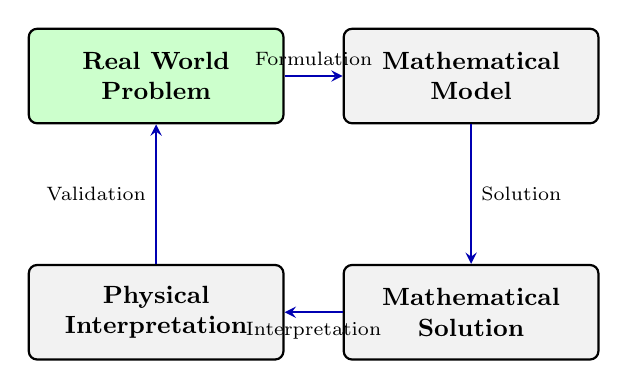
\begin{tikzpicture}[
        node distance=3cm and 2.5cm, % Adjusted distance
        auto,
        box/.style={
            draw,
            rectangle,
            rounded corners=3pt,
            text width=3cm, % Adjusted width
            text centered,
            minimum height=1.2cm, % Adjusted height
            fill=gray!10, % Generic fill
            draw=black,
            thick,
            font=\small\bfseries
        },
        arrow/.style={
            ->,
            thick,
            color=blue!70!black, % Generic arrow color
            >=stealth
        },
        label/.style={
            font=\scriptsize,
            color=black
        }
    ]
        \node (real) [box, fill=green!20] {Real World\\Problem};
        \node (math) [box, right of=real, node distance=4cm] {Mathematical\\Model}; % Increased node distance
        \node (solution) [box, below of=math, node distance=3cm] {Mathematical\\Solution};
        \node (interpret) [box, left of=solution, node distance=4cm] {Physical\\Interpretation}; % Increased node distance

        \draw[arrow] (real) -- (math) node[midway, above, label] {Formulation};
        \draw[arrow] (math) -- (solution) node[midway, right, label] {Solution};
        \draw[arrow] (solution) -- (interpret) node[midway, below, label] {Interpretation};
        \draw[arrow] (interpret) -- (real) node[midway, left, label] {Validation};
    \end{tikzpicture}
\end{center}

\subsection{Modeling Principles}
\label{ssec:modeling_principles}
Key steps in mathematical modeling:
\begin{enumerate}
    \item \textbf{Identify} the variables and parameters.
    \item \textbf{Make assumptions} to simplify the problem.
    \item \textbf{Formulate} the differential equation(s).
    \item \textbf{Solve} the equation(s) (analytically or numerically).
    \item \textbf{Interpret} the solution in physical terms.
    \item \textbf{Validate} against experimental data or known facts.
    \item \textbf{Refine} the model if necessary.
\end{enumerate}

\subsection{Example: Population Growth Model}
\label{ssec:example_population_growth}
\textbf{Problem:} Model the growth of a population over time.

\textbf{Assumptions:}
\begin{itemize}
    \item The birth rate is proportional to the current population.
    \item There are no deaths, immigration, or emigration (closed system).
    \item Resources are unlimited.
\end{itemize}

\textbf{Mathematical Model:}
Let $P(t)$ be the population at time $t$, and $r$ be the constant growth rate.
The rate of change of the population, $\frac{dP}{dt}$, is proportional to $P(t)$:
\begin{equation}
    \frac{dP}{dt} = rP \label{eq:population_growth}
\end{equation}
This is a first-order, linear, ordinary differential equation with constant coefficients.

\chapter{Linear Equations with Variable Coefficients and Separable Equations}
\label{chap:session_2}

This chapter covers the fundamental solution techniques for first-order differential equations.

\section{Linear Equations with Variable Coefficients}
\label{sec:linear_variable_coeffs}

A \textbf{first-order linear differential equation} can be written in the standard form:
\begin{equation}
    \frac{dy}{dx} + P(x)y = Q(x)
    \label{eq:book_linear_de_standard_form}
\end{equation}
where $P(x)$ and $Q(x)$ are continuous functions of $x$.

Key characteristics of this type of equation include:
\begin{itemize}
    \item The dependent variable $y$ and its derivative $\frac{dy}{dx}$ appear only to the first power.
    \item There are no products of $y$ and its derivatives (e.g., $y \cdot \frac{dy}{dx}$ or $(\frac{dy}{dx})^2$).
    \item The coefficients $P(x)$ and $Q(x)$ can be functions of the independent variable $x$.
\end{itemize}

\section{Method of Solution: Integrating Factor}
\label{sec:book_integrating_factor}
To solve the linear differential equation given by Equation~\ref{eq:book_linear_de_standard_form}, we employ the method of the integrating factor.

\subsubsection{Step 1: Calculate the Integrating Factor}
The \textbf{integrating factor}, denoted by $\mu(x)$, is defined as:
\begin{equation}
    \mu(x) = e^{\int P(x)dx}
    \label{eq:book_integrating_factor_formula}
\end{equation}
Note that the constant of integration can be omitted when calculating $\mu(x)$, as it would only introduce a multiplicative constant that cancels out later.

\subsubsection{Step 2: Multiply by the Integrating Factor}
Multiply the entire standard differential equation (Equation~\ref{eq:book_linear_de_standard_form}) by $\mu(x)$:
\begin{equation}
    \mu(x)\frac{dy}{dx} + \mu(x)P(x)y = \mu(x)Q(x)
    \label{eq:book_multiplied_by_mu}
\end{equation}
The crucial property of the integrating factor is that the left side of Equation~\ref{eq:book_multiplied_by_mu} becomes the derivative of the product $\mu(x)y$ with respect to $x$:
\begin{equation}
    \frac{d}{dx}[\mu(x)y] = \mu(x)P(x)y + \mu(x)\frac{dy}{dx}
\end{equation}
Thus, Equation~\ref{eq:book_multiplied_by_mu} can be rewritten as:
\begin{equation}
    \frac{d}{dx}[\mu(x)y] = \mu(x)Q(x)
    \label{eq:book_derivative_product_form}
\end{equation}

\subsubsection{Step 3: Integrate Both Sides}
Integrate both sides of Equation~\ref{eq:book_derivative_product_form} with respect to $x$:
\begin{equation}
    \int \frac{d}{dx}[\mu(x)y] dx = \int \mu(x)Q(x)dx
\end{equation}
This yields:
\begin{equation}
    \mu(x)y = \int \mu(x)Q(x)dx + C
    \label{eq:book_integrated_form}
\end{equation}
where $C$ is the constant of integration.

\subsubsection{Step 4: Solve for $y(x)$}
Finally, solve for $y(x)$ by dividing Equation~\ref{eq:book_integrated_form} by $\mu(x)$ (assuming $\mu(x) \neq 0$, which is true since it is an exponential):
\begin{equation}
    y(x) = \frac{1}{\mu(x)} \left( \int \mu(x)Q(x)dx + C \right)
    \label{eq:book_linear_de_solution}
\end{equation}
This is the general solution to the first-order linear differential equation.

\subsection{Example: Solving a Linear Differential Equation}
\label{ssec:book_example_linear_de}
Consider the differential equation:
\begin{equation}
    x\frac{dy}{dx} - 2y = x^2 \quad \text{for } x > 0
    \label{eq:book_ex_linear_problem}
\end{equation}

\textbf{1. Standard Form:}
To put Equation~\ref{eq:book_ex_linear_problem} into the standard form $\frac{dy}{dx} + P(x)y = Q(x)$, we divide by $x$ (which is permissible since $x > 0$):
\begin{equation}
    \frac{dy}{dx} - \frac{2}{x}y = x
    \label{eq:book_ex_linear_standard}
\end{equation}
From this, we identify $P(x) = -\frac{2}{x}$ and $Q(x) = x$.

\textbf{2. Integrating Factor $\mu(x)$:}
Calculate the integrating factor using Equation~\ref{eq:book_integrating_factor_formula}:
\begin{equation}
    \mu(x) = e^{\int -\frac{2}{x}dx}
\end{equation}
First, evaluate the integral: $\int -\frac{2}{x}dx = -2\ln|x|$. Since $x > 0$, $|x|=x$, so $-2\ln x = \ln x^{-2}$.
Therefore, the integrating factor is:
\begin{equation}
    \mu(x) = e^{\ln x^{-2}} = x^{-2} = \frac{1}{x^2}
\end{equation}

\textbf{3. Multiply by $\mu(x)$ and Integrate:}
Multiply the standard form (Equation~\ref{eq:book_ex_linear_standard}) by $\mu(x) = \frac{1}{x^2}$:
\begin{equation}
    \frac{1}{x^2}\left(\frac{dy}{dx} - \frac{2}{x}y\right) = \frac{1}{x^2} \cdot x
\end{equation}
This simplifies to:
\begin{equation}
    \frac{1}{x^2}\frac{dy}{dx} - \frac{2}{x^3}y = \frac{1}{x}
\end{equation}
The left side is $\frac{d}{dx}\left[\frac{1}{x^2}y\right]$. So, we have:
\begin{equation}
    \frac{d}{dx}\left[\frac{1}{x^2}y\right] = \frac{1}{x}
\end{equation}
Now, integrate both sides with respect to $x$:
\begin{equation}
    \frac{1}{x^2}y = \int \frac{1}{x}dx = \ln|x| + C
\end{equation}
Since $x > 0$, this becomes:
\begin{equation}
    \frac{1}{x^2}y = \ln x + C
\end{equation}

\textbf{4. Solve for $y(x)$:}
Multiply by $x^2$ to isolate $y(x)$:
\begin{equation}
    y(x) = x^2(\ln x + C)
    \label{eq:book_ex_linear_solution}
\end{equation}
This is the general solution to the given differential equation for $x > 0$.

\subsection{Separable Equations}
\label{ssec:separable_equations}

A first-order differential equation is called \textbf{separable} if it can be written in a form where all terms involving the independent variable $x$ (and $dx$) can be moved to one side of the equation, and all terms involving the dependent variable $y$ (and $dy$) can be moved to the other side.

Standard forms for separable equations are:
\begin{equation}
    M(x)dx + N(y)dy = 0
    \label{eq:book_separable_form1}
\end{equation}
or, equivalently, if the derivative $\frac{dy}{dx}$ can be expressed as a product of a function of $x$ and a function of $y$:
\begin{equation}
    \frac{dy}{dx} = f(x)g(y)
    \label{eq:book_separable_form2}
\end{equation}

\subsection{Method of Solution: Separation and Integration}
\label{ssec:book_separable_solution_method}
To solve a separable equation of the form given by Equation~\ref{eq:book_separable_form2}:

\subsubsection{Step 1: Separate Variables}
Assuming $g(y) \neq 0$, we can algebraically manipulate the equation to group $x$ terms with $dx$ and $y$ terms with $dy$:
\begin{equation}
    \frac{1}{g(y)}dy = f(x)dx
    \label{eq:book_variables_separated}
\end{equation}
If there are values of $y$ for which $g(y)=0$, these may represent constant (equilibrium) solutions that should be checked separately.

\subsubsection{Step 2: Integrate Both Sides}
Integrate both sides of Equation~\ref{eq:book_variables_separated} with respect to their respective variables:
\begin{equation}
    \int \frac{1}{g(y)}dy = \int f(x)dx + C
    \label{eq:book_separable_integrated}
\end{equation}
where $C$ is the constant of integration. It is customary to add the constant of integration to the side involving the independent variable $x$.

\subsubsection{Step 3: Solve for $y(x)$ (if possible)}
The result of the integration in Equation~\ref{eq:book_separable_integrated} is often an implicit solution relating $x$ and $y$. If possible and desired, one can attempt to solve this equation explicitly for $y(x)$.

\subsection{Example: Solving a Separable Differential Equation}
\label{ssec:book_example_separable_de}
Consider the differential equation:
\begin{equation}
    \frac{dy}{dx} = \frac{x^2}{y^2}
    \label{eq:book_ex_separable_problem}
\end{equation}

\textbf{1. Separate Variables:}
Multiply both sides by $y^2$ and $dx$ to separate the variables (assuming $y \neq 0$):
\begin{equation}
    y^2 dy = x^2 dx
\end{equation}

\textbf{2. Integrate Both Sides:}
Integrate both sides with respect to their respective variables:
\begin{equation}
    \int y^2 dy = \int x^2 dx
\end{equation}
Performing the integration yields:
\begin{equation}
    \frac{y^3}{3} = \frac{x^3}{3} + C_1
\end{equation}
where $C_1$ is the constant of integration.

\textbf{3. Solve for $y(x)$ (optional form):}
To obtain an explicit solution for $y$, multiply by 3:
\begin{equation}
    y^3 = x^3 + 3C_1
\end{equation}
Let $C = 3C_1$ (since $C_1$ is an arbitrary constant, $3C_1$ is also an arbitrary constant). Then:
\begin{equation}
    y^3 = x^3 + C
\end{equation}
Finally, take the cube root of both sides:
\begin{equation}
    y(x) = \sqrt[3]{x^3 + C}
    \label{eq:book_ex_separable_solution}
\end{equation}
This is the general solution to the given separable differential equation. Note that $y=0$ was excluded in the separation step; however, $y(x)=0$ is not a solution to the original DE.

\chapter{Modeling with First-Order Equations}
\label{chap:session_3}
% Session 3 content: Modeling with first-order equations and physical applications

\textit{This chapter will cover:}
\begin{itemize}
    \item Mathematical modeling principles applied to first-order DEs
    \item Population dynamics models (exponential and logistic growth)
    \item Newton's law of cooling/heating
    \item Mixing problems and compartmental analysis
    \item RC circuit applications
    \item Physical interpretation of solutions
\end{itemize}

\chapter{Problem-Solving Workshop}
\label{chap:session_4}
% Session 4 content: Practice problems and case studies

\textit{This chapter will include:}
\begin{itemize}
    \item Complex modeling exercises
    \item Case studies involving first-order DEs
    \item Step-by-step solution techniques
    \item Model validation and interpretation
    \item Real-world applications and examples
\end{itemize}

% ============================================================================
% PART II: MODULE 2 - SECOND-ORDER DIFFERENTIAL EQUATIONS (Sessions 5-7)
% ============================================================================
\part{Second-Order Differential Equations}
\label{part:second_order_de}

\chapter{Introduction to Oscillations and Fundamental Solutions}
\label{chap:session_5}
% Session 5 content

\textit{This chapter will cover:}
\begin{itemize}
    \item Introduction to oscillatory motion
    \item Linear differential operators
    \item Fundamental solutions of homogeneous equations
    \item Characteristic equations and their roots
    \item Physical interpretation of oscillatory solutions
\end{itemize}

\chapter{Homogeneous and Non-Homogeneous Equations}
\label{chap:session_6}
% Session 6 content

\textit{This chapter will cover:}
\begin{itemize}
    \item Homogeneous linear equations with constant coefficients
    \item Complex auxiliary equations and complex roots
    \item Superposition principle
    \item Non-homogeneous equations and particular solutions
    \item Method of undetermined coefficients
\end{itemize}

\chapter{Applied Mathematical Modeling}
\label{chap:session_7}
% Session 7 content (Practice)

\textit{This chapter will include:}
\begin{itemize}
    \item Vibrations and oscillatory motion problems
    \item Method of undetermined coefficients
    \item Variation of parameters method
    \item Practical applications and examples
    \item Problem-solving techniques
\end{itemize}

% ============================================================================
% PART III: MODULE 3 - POWER SERIES SOLUTIONS AND SPECIAL FUNCTIONS (Sessions 8-10)
% ============================================================================
\part{Power Series Solutions and Special Functions}
\label{part:power_series_special_functions}

\chapter{Power Series and Taylor Series Solutions}
\label{chap:session_8}
% Session 8 content

\textit{This chapter will cover:}
\begin{itemize}
    \item Power series and analytic functions
    \item Taylor series solutions to differential equations
    \item Solutions in power series of linear differential equations
    \item Convergence and radius of convergence
    \item Applications to physics and engineering
\end{itemize}

\chapter{Cauchy-Euler Equations and Frobenius Method}
\label{chap:session_9}
% Session 9 content

\textit{This chapter will cover:}
\begin{itemize}
    \item Cauchy-Euler equations
    \item Classification of singular points
    \item Frobenius method for series solutions
    \item Orthogonal polynomials
    \item Special functions (Bessel, Legendre, etc.)
\end{itemize}

\chapter{Applications of Special Functions}
\label{chap:session_10}
% Session 10 content (Practice)

\textit{This chapter will include:}
\begin{itemize}
    \item Special functions applications in physics
    \item Series solution techniques
    \item Obtaining linearly independent solutions
    \item Boundary value problems
    \item Practical problem-solving
\end{itemize}

% ============================================================================
% PART IV: MODULE 4 - LAPLACE TRANSFORM METHODS (Sessions 11-13)
% ============================================================================
\part{Laplace Transform Methods}
\label{part:laplace_transforms}

\chapter{Definition and Properties of Laplace Transforms}
\label{chap:session_11}
% Session 11 content

\textit{This chapter will cover:}
\begin{itemize}
    \item Definition of the Laplace transform
    \item Properties and basic transforms
    \item Solution of initial value problems
    \item Transform of derivatives and integrals
    \item Inverse Laplace transforms
\end{itemize}

\chapter{Convolution and Step Functions}
\label{chap:session_12}
% Session 12 content

\textit{This chapter will cover:}
\begin{itemize}
    \item Convolution theorem and Abel problem
    \item Unit step function (Heaviside function)
    \item Impulse function (Dirac delta)
    \item Applications to engineering problems
    \item Transfer functions
\end{itemize}

\chapter{Transform Method Applications}
\label{chap:session_13}
% Session 13 content (Practice)

\textit{This chapter will include:}
\begin{itemize}
    \item Complex problem-solving using Laplace transforms
    \item Systems of differential equations
    \item Engineering applications
    \item Circuit analysis problems
    \item Mechanical vibration problems
\end{itemize}

% ============================================================================
% PART V: MODULE 5 - NON-LINEAR DIFFERENTIAL EQUATIONS (Sessions 14-16)
% ============================================================================
\part{Non-Linear Differential Equations}
\label{part:nonlinear_de}

\chapter{Autonomous Systems and Phase Portraits}
\label{chap:session_14}
% Session 14 content

\textit{This chapter will cover:}
\begin{itemize}
    \item Autonomous systems of differential equations
    \item Critical points and equilibrium solutions
    \item Stability analysis techniques
    \item Phase portraits for linear systems
    \item Classification of critical points
\end{itemize}

\chapter{Non-Linear Stability and Lyapunov Method}
\label{chap:session_15}
% Session 15 content

\textit{This chapter will cover:}
\begin{itemize}
    \item Stability of non-linear systems
    \item Lyapunov's direct method
    \item Lyapunov functions and stability criteria
    \item Periodic solutions
    \item Poincaré-Bendixon theorem
\end{itemize}

\chapter{Phase Portrait Construction and Applications}
\label{chap:session_16}
% Session 16 content (Practice)

\textit{This chapter will include:}
\begin{itemize}
    \item Phase portrait construction techniques
    \item Stability analysis problems
    \item Non-linear system modeling
    \item Predator-prey models
    \item Engineering applications
\end{itemize}

% ============================================================================
% PART VI: MODULE 6 - PARTIAL DIFFERENTIAL EQUATIONS (Sessions 17-19)
% ============================================================================
\part{Partial Differential Equations}
\label{part:partial_de}

\chapter{Separation of Variables and Sturm-Liouville Problems}
\label{chap:session_17}
% Session 17 content

\textit{This chapter will cover:}
\begin{itemize}
    \item Variable separation method for PDEs
    \item Sturm-Liouville boundary value problems
    \item Eigenvalues and eigenfunctions
    \item Orthogonality of eigenfunctions
    \item Applications to physics problems
\end{itemize}

\chapter{Heat, Wave, and Laplace Equations}
\label{chap:session_18}
% Session 18 content

\textit{This chapter will cover:}
\begin{itemize}
    \item The heat equation (diffusion equation)
    \item The wave equation
    \item Laplace's equation (potential theory)
    \item Boundary and initial conditions
    \item Physical interpretation of solutions
\end{itemize}

\chapter{PDE Solution Methods and Applications}
\label{chap:session_19}
% Session 19 content (Practice)

\textit{This chapter will include:}
\begin{itemize}
    \item Advanced PDE solution techniques
    \item Boundary value problems in engineering
    \item Laplace transform methods for PDEs
    \item Fourier series applications
    \item Practical problem-solving
\end{itemize}

% ============================================================================
% COMPREHENSIVE REVIEW (Session 20)
% ============================================================================

\chapter{Comprehensive Review and Integration}
\label{chap:session_20}
% Session 20 content

\textit{This chapter will include:}
\begin{itemize}
    \item Integration of all course topics
    \item Key concepts synthesis
    \item Problem-solving strategies overview
    \item Connections between different DE types
    \item Mathematical modeling competency review
\end{itemize}

\appendix
\chapter{Assessment Framework (Conceptual)}
\label{app:assessment}
While this book serves as a textual resource, the original course assessment was structured as:
\begin{itemize}
    \item \textbf{50\% Cumulative Theoretical-Practical Midterm Examinations}
    \begin{itemize}
        \item After modules 2, 4, and 6 (sessions 7, 13, 19)
    \end{itemize}

    \item \textbf{20\% Activities, Assignments, and Integrating Cases}
    \begin{itemize}
        \item During practice sessions (4, 7, 10, 13, 16, 19)
    \end{itemize}

    \item \textbf{30\% Final Integrating Examination}
    \begin{itemize}
        \item Session 20 (comprehensive assessment)
    \end{itemize}
\end{itemize}
For self-study, readers are encouraged to work through examples and exercises provided in each chapter.

\chapter{Recommended Texts and Further Reading}
\label{app:texts}
\textbf{Primary Text (basis for much of this material):}
\begin{itemize}
    \item Nagle, R. Kent, Saff, Edward B., Snider, Arthur David. \textit{Fundamentals of Differential Equations and Boundary Value Problems}, 9th ed. Pearson, 2018. (Updated from original reference)
\end{itemize}

\textbf{Supplementary References:}
\begin{itemize}
    \item Simmons, George F. \textit{Differential Equations with Applications and Historical Notes}, 3rd ed. CRC Press, 2017.
    \item Boyce, William E., DiPrima, Richard C., Meade, Douglas B. \textit{Elementary Differential Equations and Boundary Value Problems}, 11th ed. Wiley, 2017.
    \item Zill, Dennis G. \textit{A First Course in Differential Equations with Modeling Applications}, 11th ed. Cengage Learning, 2018.
\end{itemize}

\backmatter % For bibliography, index, etc.
% \bibliography{references} % If you have a .bib file
% \bibliographystyle{plain}

% Placeholder for a simple bibliography if not using BibTeX
\begin{thebibliography}{9}
    \bibitem{nagle2018} Nagle, R. K., Saff, E. B., \& Snider, A. D. (2018). \textit{Fundamentals of Differential Equations and Boundary Value Problems} (9th ed.). Pearson.
    \bibitem{simmons2017} Simmons, G. F. (2017). \textit{Differential Equations with Applications and Historical Notes} (3rd ed.). CRC Press.
    \bibitem{boyce2017} Boyce, W. E., DiPrima, R. C., \& Meade, D. B. (2017). \textit{Elementary Differential Equations and Boundary Value Problems} (11th ed.). Wiley.
    \bibitem{zill2018} Zill, D. G. (2018). \textit{A First Course in Differential Equations with Modeling Applications} (11th ed.). Cengage Learning.
\end{thebibliography}

\end{document}
